\subsection{Bild 1 - Kashvi am Brett}
\begin{center}
    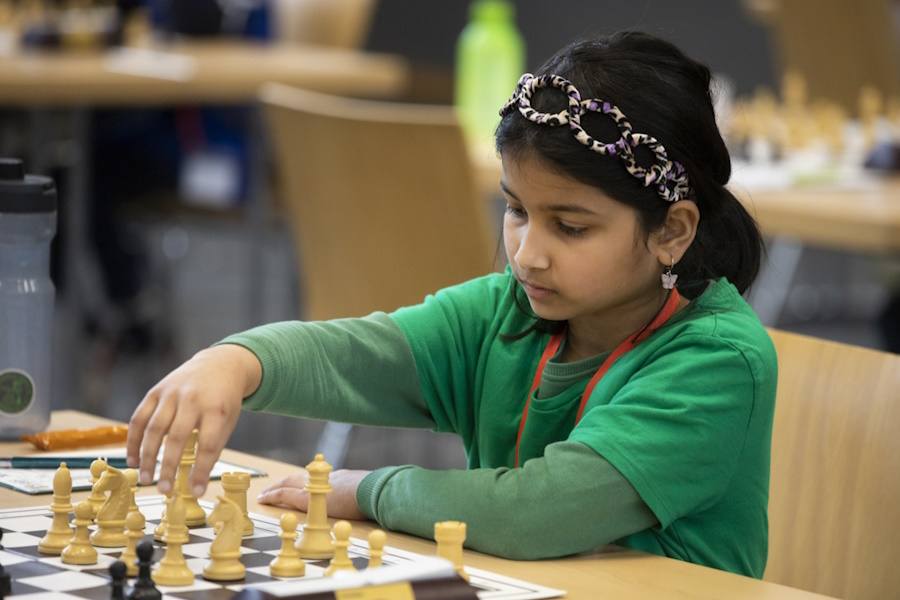
\includegraphics[width=\linewidth,height=0.5625\linewidth,keepaspectratio]{THJEM2.jpg}
    \captionof{figure}{Kashvi Bild}
    \label{fig:Kashvi Bild}
\end{center}

\subsection{Bild 2 - Hanna gegen Anna in Runde 1}
\begin{center}
    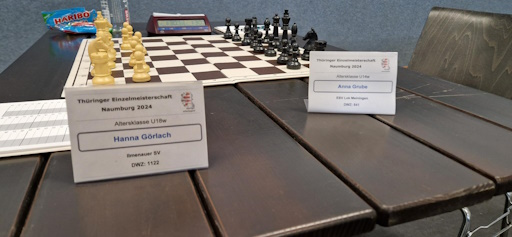
\includegraphics[width=0.8\linewidth,height=0.45\linewidth,keepaspectratio]{THJEM1.jpeg}
    \captionof{figure}{THJEM Hanna Schild}
    \label{fig:THJEM Hanna Schild}
\end{center}

\clearpage
\section{Partie von Kashvi}
% TODO: PGN der Analysierten Partie einfügen